\section{Nierozstrzygalność}

\subsection{Pierwsze twierdzenie Rice'a}

Dla \( S \subseteq RE \) definiujemy \( L_S = \set{\langle M \rangle : L(M) \in S} \). \\
Własność \(S\) jest trywialna, jeśli \(S = \emptyset \) lub \(S = RE\). Takie własności są rozstrzygalne -- jeśli \(S = \emptyset\), to \( L_S = \emptyset \) i jest rozpoznawana przez maszynę z własnością STOP, która odrzuca wszystkie słowa, a jeśli \(S = RE\), to \(L_S\) zawiera wszystkie poprawne kody maszyn, więc do rozpoznania \(L_S\) wystarczy parser.

\begin{theorem}{(Rice)}
    Każda nietrywialna własność języków rekurencyjnie przeliczalnych jest nierozstrzygalna, czyli poza Rec.
\end{theorem}
\begin{proof}
    Niech \(S\) będzie nietrywialną własnością. Załóżmy, że \( \emptyset \notin S \). Możemy tak zrobić, ponieważ dopełnienie nietrywialnej własności również jest nietrywialne, więc jeśli \( \emptyset \in S \) prowadzimy analogiczne rozumowanie dla dopełnienia \(S\).

    Niech \( L_0 = L(M_0) \in S \). Dla dowodu nie wprost załóżmy, że \( S \) jest rozstrzygalna. Konstruujemy maszynę \(N\) z własnością stopu:
    \begin{figure}[H]
        \centering
        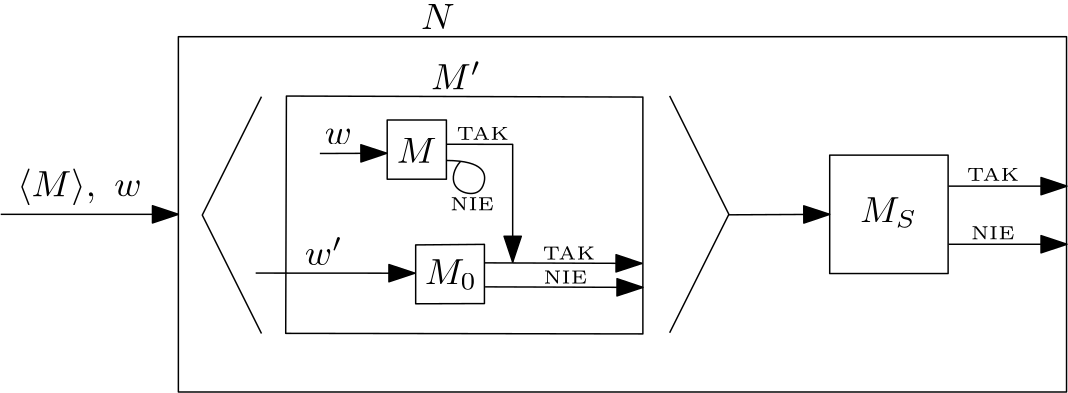
\includegraphics[width=0.75\linewidth]{img/rice.png}
    \end{figure}
    Jeśli \(M\) akceptuje \(w\), to \(L(M') = L_0\), więc \(M_S\) akceptuje. W przeciwnym przypadku \(L(M') = \emptyset\), więc \(M_S\) nie akceptuje z założenia, że \(\emptyset \notin S\). Maszyna \(N\) rozpoznaje język \(L_U\), który nie jest rozstrzygalny -- sprzeczność.
\end{proof}


\subsection{Drugie twierdzenie Rice'a}

\subsection*{Monotoniczność}
\vspace{-0.8em}
\[ (L \in S \land L \subset L' \in RE)\Longleftrightarrow L' \in S \]
\vspace{-1em}
\begin{lemma}
    Jeśli \(S\) nie jest monotoniczna, to \(L_S \notin RE\).
\end{lemma}
\begin{proof}
    Nie wprost załóżmy, że \(S\) nie jest monotoniczna oraz \(L_S \in RE\). Istnieje maszyna \(M_S\), która rozpoznaje \(L_S\).

    Weźmy \(L_1 \subset L_2\), takie że \(L_1 \in S, L_2 \notin S\) oraz są rozpoznawane przez maszyny \(M_1, M_2\).
    \vspace{-0.8em}
    \begin{figure}[H]
        \centering
        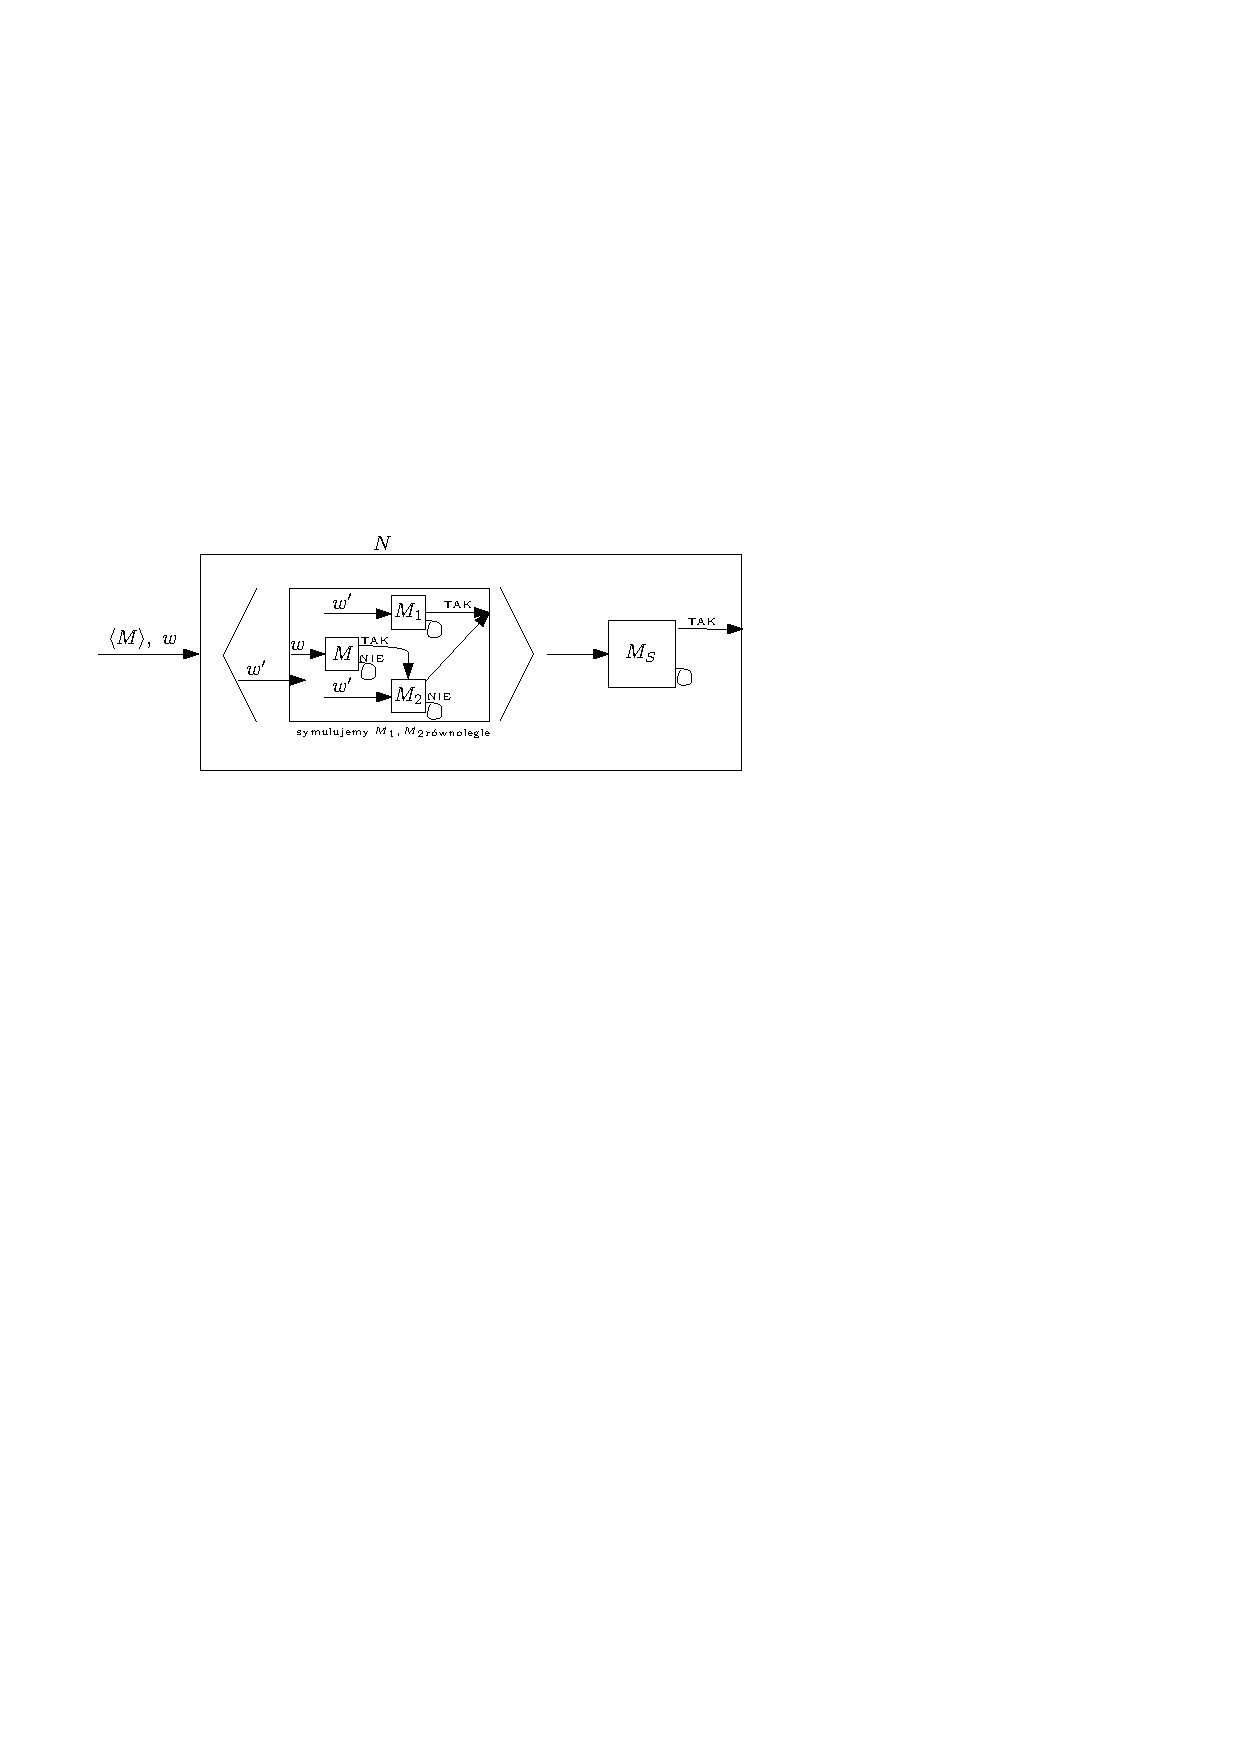
\includegraphics[width=0.75\linewidth]{img/monotoniczność.pdf}
    \end{figure}
    \vspace{-0.8em}
    Symulujemy \(M_1, M_2\) równolegle. Jeśli \(M\) akceptuje \(w\), to \(L(M')=L_2\). Jeśli nie akceptuje, to \(L(M')=L_1\), więc \(M_s\) akceptuje. Zatem \(N\) rozpoznaje \(\overline{L_U}\) -- sprzeczność.
\end{proof}

\subsection*{Własność skończonego podjęzyka}
\[ \forall_{L \in S} \ \exists_{L' \:\subseteq\: L} \ L' \in S \land L' \text{ skończony} \]

\begin{lemma}
    Jeśli \(S\) nie ma własności skończonego podjęzyka, to \(L(S)\notin RE\).
\end{lemma}
\begin{proof}
    Nie wprost załóżmy, że \( L\in S\)  i nie ma własności skończonego podjęzyka.
    \vspace{-0.8em}
    \begin{figure}[H]
        \centering
        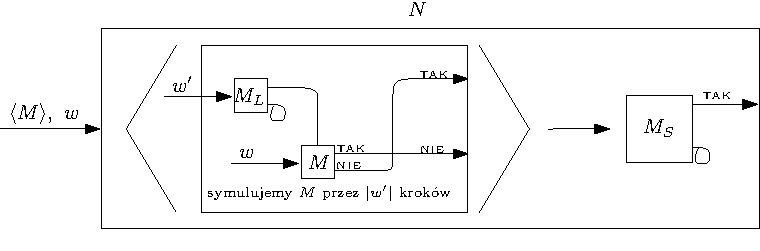
\includegraphics[width=0.75\linewidth]{img/skonczony-podjezyk.pdf}
    \end{figure}
    \vspace{-0.8em}
    Jeśli \(M\) akceptuje \(w\) w \(k\) krokach, to \(L(M') = L \cap \set{w \: :|w|<k}\), czyli skończony podjęzyk \(L\). Ponieważ \(S\) nie ma własności skończonego podjęzyka, to \(N\) się zapętli.

    Jeśli \(M\) nie akceptuje \(w\), to \(L(M') = L \in S\) i \(N\) akceptuje. Czyli \(N\) rozpoznaje \(\overline{L_U}\) -- sprzeczność.
\end{proof}


\subsection*{Uniwersalność}
Klasa skończonych języków \(S\) jest uniwersalna, jeśli istnieje maszyna Turinga (numerator) bez wejścia, wypisująca suriektywnie języki skończone z \(S\).
\[code_1 \# code_2 \# code_3 \# \dots \qquad code_i = w_1 \$ w_2 \$ \dots \$ w_p\]

\newpage
\begin{lemma}{(O numeratorze)}
    Jeśli \(S \subset RE\), to istnieje numerator dla skończonych języków z \(S\).
\end{lemma}
\begin{proof}
    Przechodzimy po \((i,j) \in \mathbb{N}^2 \) przekątniowo. Maszyna \(K\), dostawszy kod skończonego języka \(L\), zwraca maszynę \(M_L\), która go rozpoznaje.
    \begin{figure}[ht!]
        \centering
        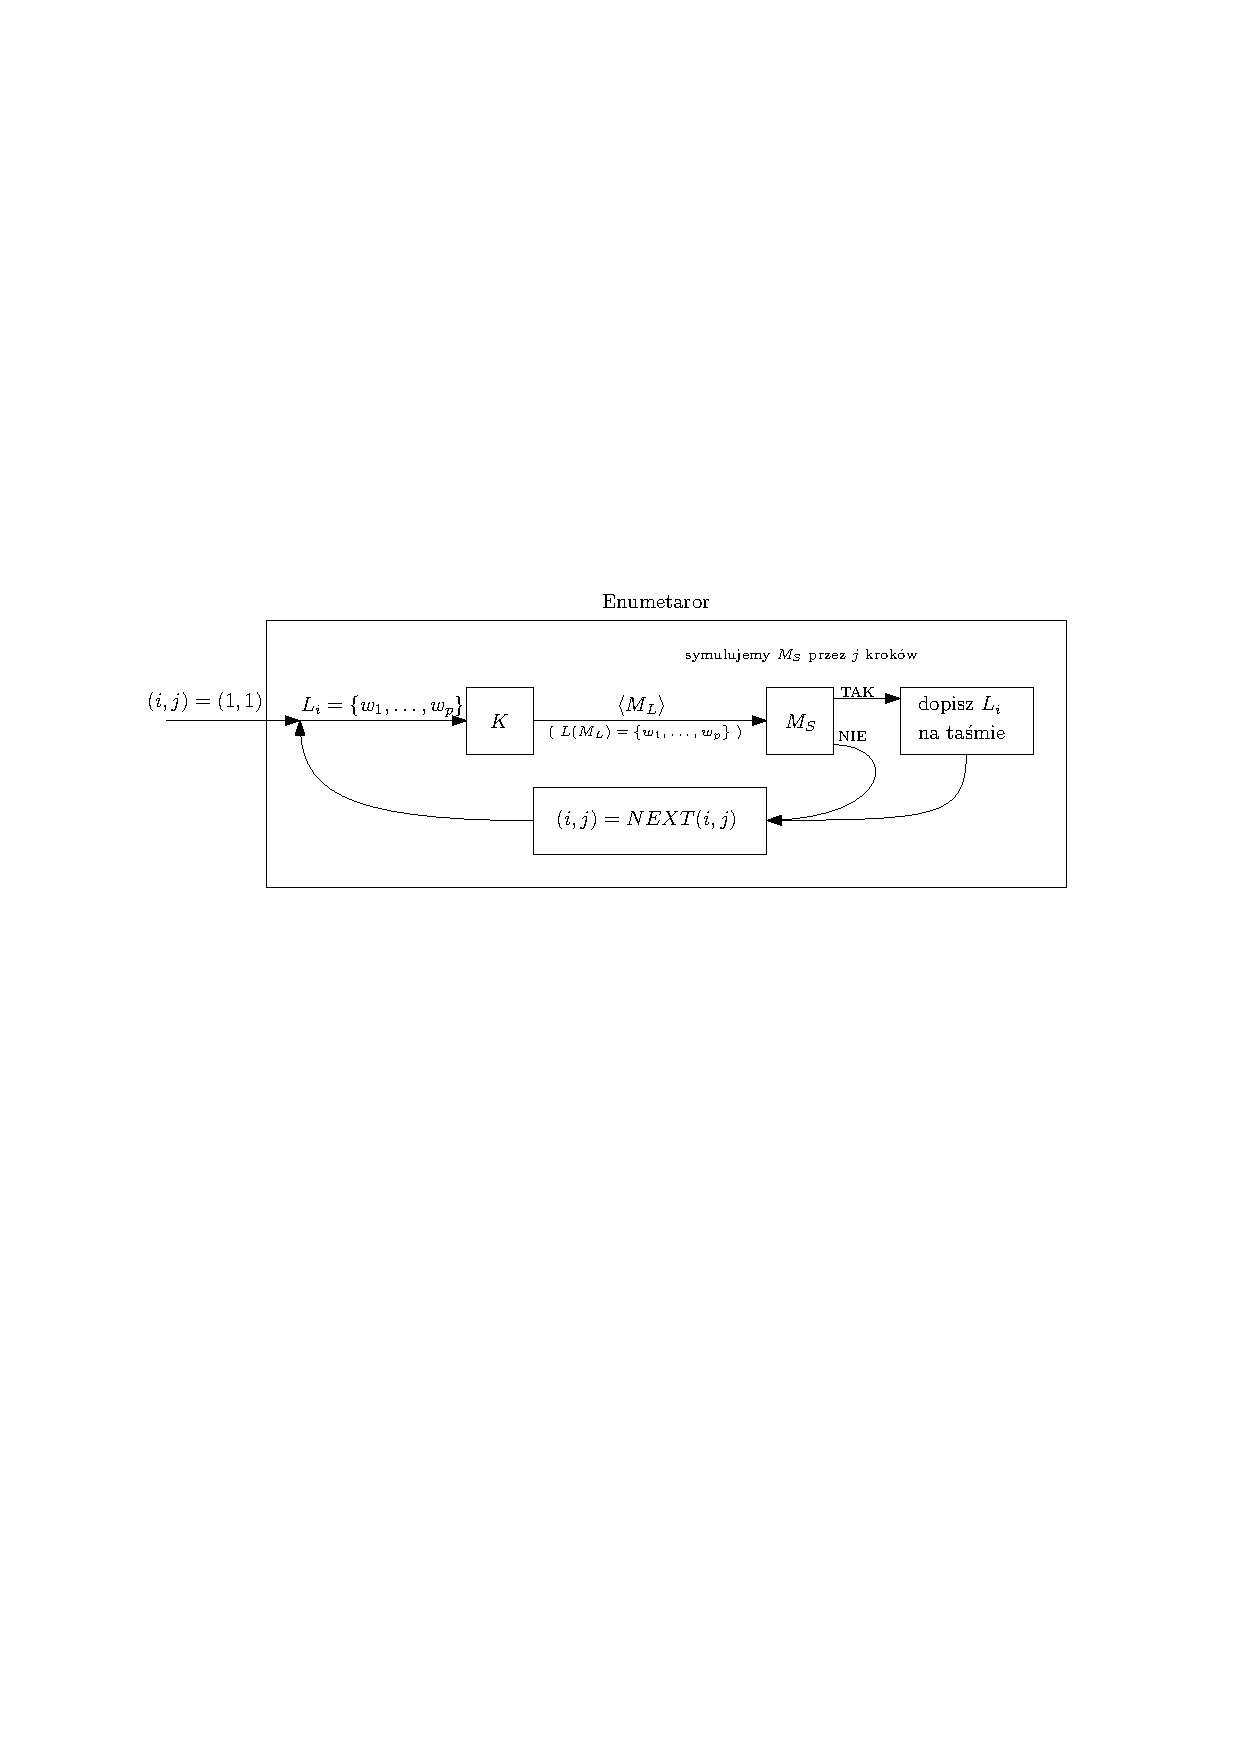
\includegraphics[width=1\linewidth]{img/enumerator.pdf}
    \end{figure}
\end{proof}

\begin{theorem}{(Rice)}
    Język \(L_S=\set{\langle M \rangle: L(M) \in S}\) jest w klasie \(RE\) wtw \(S\) jest monotoniczna, uniwersalna i ma własność skończonego podjęzyka.
\end{theorem}
\begin{proof}
    Jeśli \(L_S \in RE\), to warunki są spełnione, co wynika z lematów.
    
    Dowodzimy, że jeśli warunki są spełnione, to \(L_S \in RE\). Konstruujemy rozpoznawacza \(M_S\).

    Na wejściu jest \(\langle M \rangle\) z numeratorem \(M_{\text{NUM}}\). Przechodzimy przekątnymi po \((i,j)\).
    \begin{enumerate}
        \item Wykonujemy \(i\) kroków \(M_{\text{NUM}}\). Oznaczamy ostatni kompletny wypisany język na taśmie jako \( L = \{w_1,\dots, w_p\} \).
        \item Każde ze słów \(w_1, \dots, w_p\) sprawdzamy przez \(j\) kroków na maszynie \(M\).
        \item Jeśli \(M\) akceptuje wszystkie, to zatrzymujemy maszynę i akceptujemy \(M\).
        \item Jeśli nie, to wracamy do początku z \((i,j) = \text{NEXT}(i,j)\).
    \end{enumerate}
    Jeżeli \(L(M) \in S\), to \(M_S\) się zatrzymuje i akceptuje \(M\), bo akceptuje jakiś skończony podjęzyk \(L(M)\). Jeśli \(M_S\) się zatrzymuje i akceptuje, to \(L(M) \in S\) z monotoniczności.
\end{proof}

Każda z własności jest niezależna -- dwie pozostałe jej nie implikują.